\tikzsetexternalprefix{tikz/}	% set subfolder
\tikzsetnextfilename{ADF_scheme}
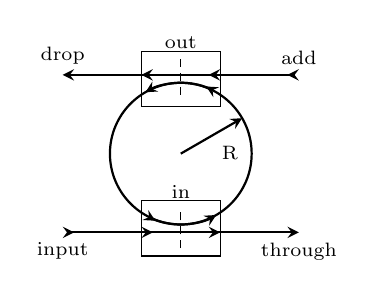
\begin{tikzpicture}[baseline, thick, every node/.style={font=\scriptsize}]
	% lowe line & arrows
	\draw [{stealth[reversed]}-stealth] (-0.5,0) -- (+0.5,0);
	% lower long line
	\draw [{stealth[reversed]}-stealth] (-1.5,0)
				node [below] {input} -- (1.5,0)
				node [below] {through};
	% lower ring
	\draw [-{stealth}] (0,0.1)
				arc [start angle=-90,end angle=-60, radius=0.9];
	\draw [-{stealth[reversed]}] (0,0.1)
				arc [start angle=-90,end angle=-120, radius=0.9];
	% lower box
	\draw [thin, densely dashed] (0,-0.2) -- (0,0.3);	
	\draw [thin]		(-0.5,0.4) -- (+0.5,0.4) --
								(+0.5,-0.3) -- (-0.5,-0.3) -- cycle;
	\node at (0, 0.3) [above] {in};

	% circle
	\draw (0,1) circle (0.9);
	% radius arrow
	\draw [-{stealth}] (0,1)
				-- ++(30:0.9cm) node [midway, below right] {R};

	% upper lines & arrows
	\draw [{stealth[reversed]}-stealth] (+0.5,2) -- (-0.5,2);
	% upper long line
	\draw [{stealth[reversed]}-stealth] (+1.5,2)
				node [above] {add} -- (-1.5,2)
				node [above] {drop};
	% upper ring
	\draw [-{stealth[reversed]}] (0,1.9)
				arc [start angle=+90,end angle=+60, radius=0.9];
	\draw [-{stealth}] (0,1.9)
				arc [start angle=+90,end angle=+120, radius=0.9];
	% upper box
	\draw [thin, densely dashed] (0,2.2) -- (0,1.7);	
	\draw [thin]		(-0.5,1.6) -- (+0.5,1.6) --
								(+0.5,2.3) -- (-0.5,2.3) -- cycle;
	\node at (0, 2.2) [above] {out};
\end{tikzpicture}